\documentclass[final,t]{beamer}
\mode<presentation>{\usetheme{I6dv}}
\setbeamerfont{itemize}{size=\normalsize}
\setbeamerfont{itemize/enumerate body}{size=\normalsize}
\setbeamerfont{itemize/enumerate subbody}{size=\normalsize}
\usepackage{amsmath,amsthm,amssymb,latexsym}
\usepackage[english]{babel}
\usepackage[orientation=portrait,scale=1.78]{beamerposter}
\usepackage{mdframed}
\usepackage{tikz}
\usetikzlibrary{calc,arrows.meta,positioning,decorations.pathreplacing}

\usepackage{fancyvrb,color}
\usepackage{subcaption}

%\usepackage{pygmentsdefs}

\def\meta/{\textsc{MeTA}}
\definecolor{answerbg}{rgb}{0.87,0.929,0.996}

\newtheorem{proposedanswer}{Proposed Answer}

\newcommand{\msp}[0]{\\[0.5\baselineskip]}
\newcommand{\vsp}[0]{\vspace{0.165in}}

\newcommand{\textretrieval}{textretrieval-001}

\title{Modeling MOOC Student Behavior with Two-Layer Hidden Markov Models}
\author{Chase Geigle and ChengXiang Zhai}
\institute[University of Illinois]{University of Illinois at
Urbana-Champaign, Department of Computer Science}
\date{}

\begin{document}
\begin{frame}[fragile]
  \begin{columns}[t]
    \begin{column}{0.6\textwidth}
      \begin{block}{Why Use a Two-Layer Hidden Markov Model (TL-HMM)?}
        \begin{itemize}
          \item Student behavior is complicated $\rightarrow$ assuming
            \textbf{latent states} allows \textbf{data} to inform the
            behavior patterns we discover (rather than handwritten rules)
            \msp{}

          \item Student behavior varies over time $\rightarrow$ modeling
            \textbf{behavior transitions} between the latent states is
            important
            \msp{}

          \item Behavior analysis requires flexible time granularity
            $\rightarrow$ model allows for this \textbf{granularity to be
            chosen flexibly} so as to allow modeling behavior patterns over
            different time resolutions
        \end{itemize}
      \end{block}
      \vsp{}
      \begin{block}{Generative Process}
        \begin{itemize}
          \item Student behavior is chunked into \textbf{sessions} with
            flexible granularity (activity gap of $>10$ hours used in our
            study). \msp{}
          \item Within a session, students take actions from an
            \textbf{action set} $\mathbf{A}$.
            \msp{}
          \item Each session is viewed as being ``generated'' from a
            \textbf{latent state} $u$; this generative process is a random
            walk of the Markov model associated with state $u$.
            \msp{}
          \item Between sessions, users \textbf{transition between latent
            states} following another Markov process (hence ``two-layer'').
        \end{itemize}
      \end{block}
      \vsp{}
      \begin{block}{Transitions Between Latent States}
        \begin{figure}
          \centering
          \begin{subfigure}[t]{0.32\textwidth}
            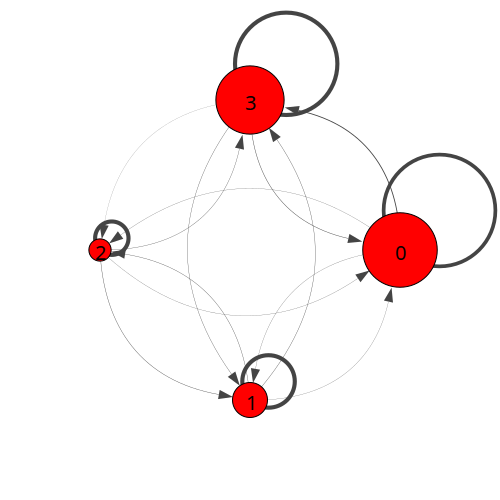
\includegraphics[width=\textwidth,trim={0 2cm 0 0cm}]{../../figures/trans-comp/trans-avg.png}
            \caption{\label{fig:trans-avg}}
          \end{subfigure}%
          \begin{subfigure}[t]{0.32\textwidth}
            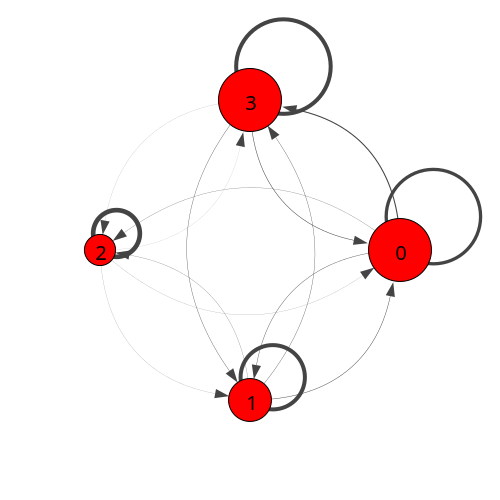
\includegraphics[width=\textwidth,trim={0 2cm 0 0cm}]{../../figures/trans-comp/trans-perfect.png}
            \caption{\label{fig:trans-perfect}}
          \end{subfigure}%
          \begin{subfigure}[t]{0.32\textwidth}
            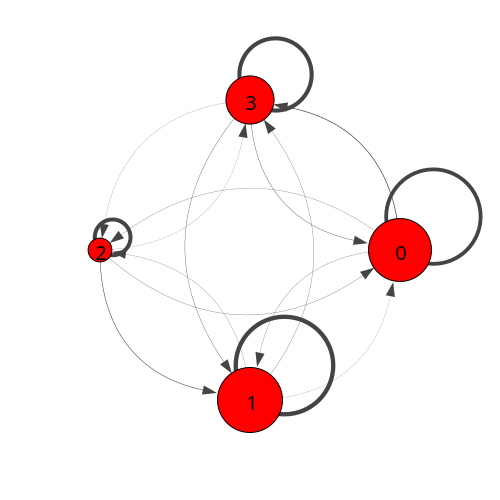
\includegraphics[width=\textwidth,trim={0 2cm 0 0cm}]{../../figures/trans-comp/trans-low.png}
            \caption{\label{fig:trans-low}}
          \end{subfigure}
          \caption{The latent state transition diagrams for a 4-state TL-HMM fit to
            \protect\textretrieval{} for all students (a) compared to only ``perfect''
          students (b) and only ``low'' students (c).}
          \label{fig:trans-comp}
        \end{figure}
      \end{block}
      \vsp{}
      \begin{block}{Latent Variables of Interest: The Two Layers}
        Individual \textbf{latent state representations} (right) and
        \textbf{transitions between them} (above). Data: 18,941 students,
        85,240 sequences, avg.\ length of 7.31.
        \begin{itemize}
          \item Size of node $\propto$ probability of visiting during
            random walk
          \item Thickness of edge $\propto$ probability of taking that edge
            from the source node
          \item Parameters learned using modified Baum-Welch
            algorithm\msp{}
        \end{itemize}
        \textbf{Right}:
        \begin{itemize}
          \item Compare state 1 vs state 3: state 1 indicates more varied
            activity during quiz taking (bottom right forum related states
            and transitions) where state 3 indicates more ``pure'' quiz
            taking.
          \item State 2: forum activity\msp{}
        \end{itemize}
        \textbf{Above:}
        \begin{itemize}
          \item ``Perfect'' (b): 100\% on all quizzes
          \item ``Low'' (c): $< 70\%$ on all quizzes (completed all)
          \item Compare: state 1 prevalence (b) vs (c); state 3 prevalence
            (b) vs (c); state 2 prevalence (a) vs (b); state 2
            $\rightarrow$ 1 transition (b) vs (c)
        \end{itemize}
      \end{block}
    \end{column}
    \begin{column}{0.3\textwidth}
      \begin{block}{Latent State Representations}
        \begin{figure}
          \centering
          \begin{subfigure}[t]{0.9\textwidth}
            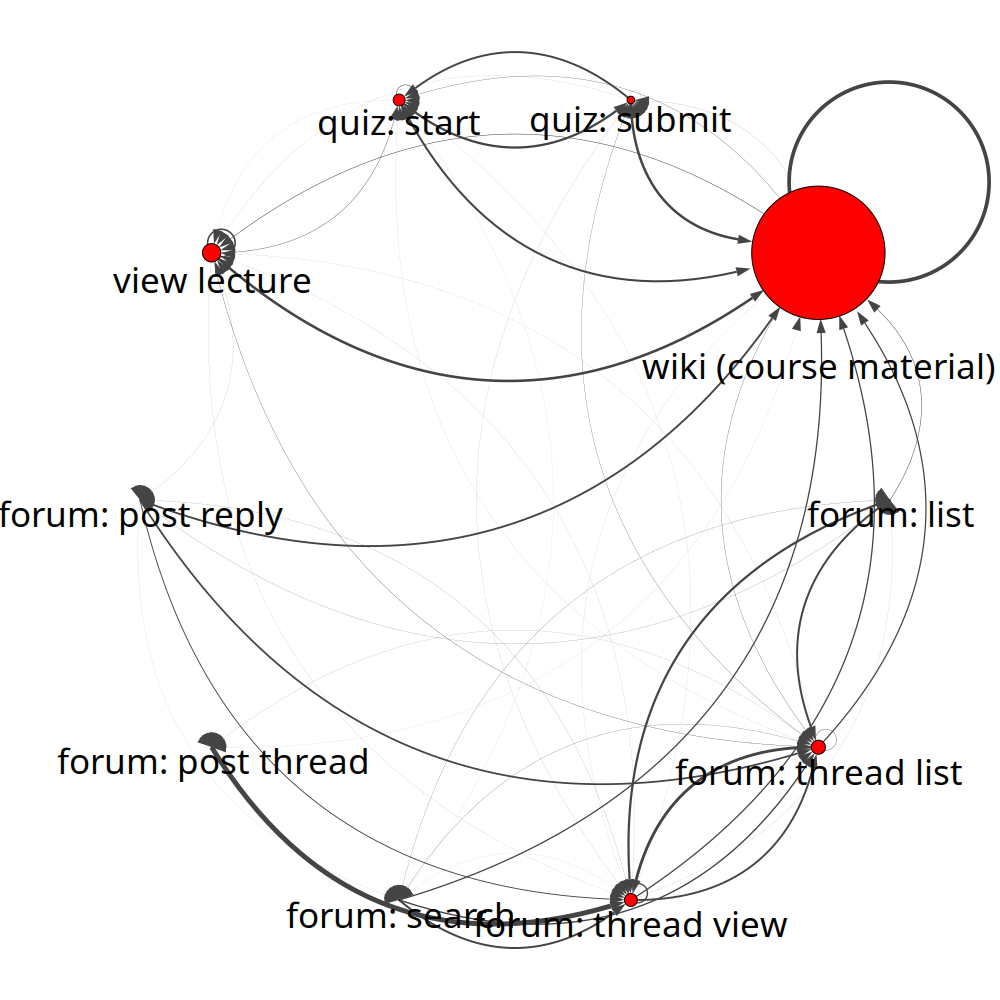
\includegraphics[width=\textwidth]{../../figures/text-4state/state0.png}
            \caption{\label{fig:state0}State 0}
          \end{subfigure}

          \begin{subfigure}[t]{0.9\textwidth}
            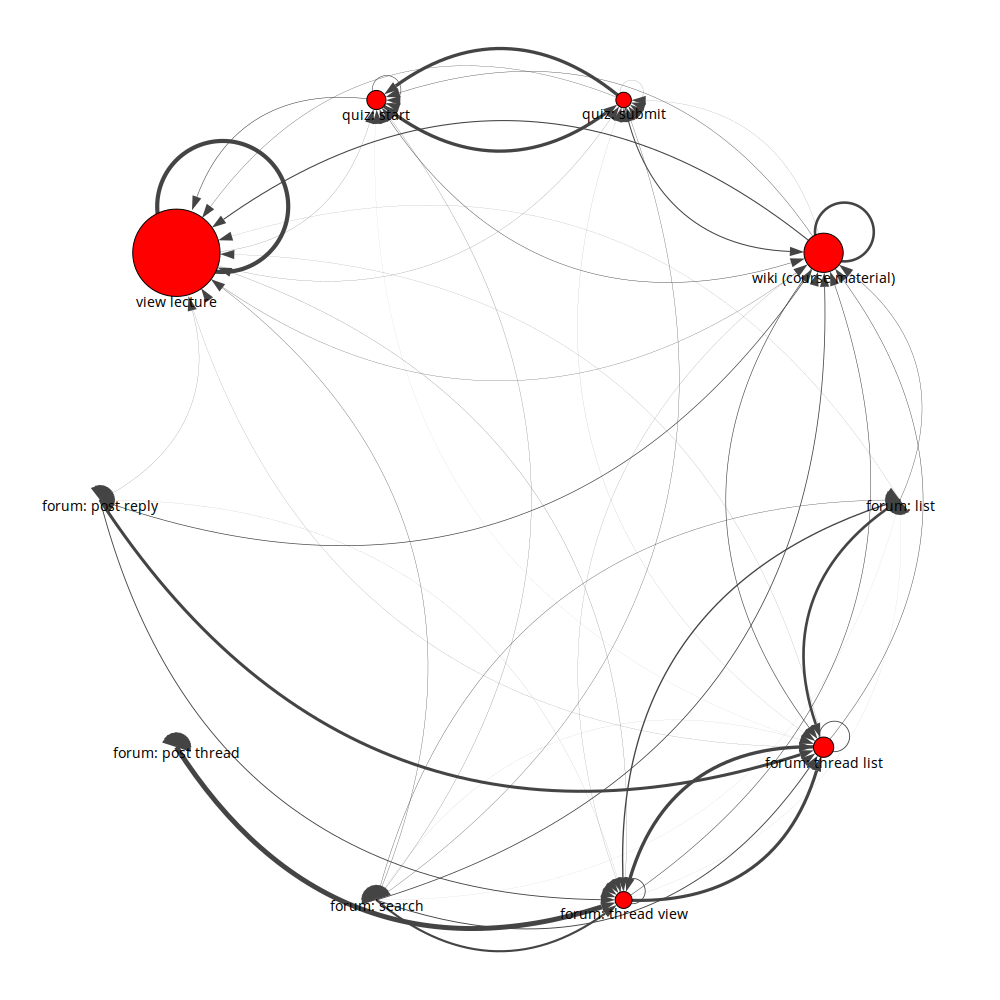
\includegraphics[width=\textwidth]{../../figures/text-4state/state1.png}
            \caption{\label{fig:state1}State 1}
          \end{subfigure}

          \begin{subfigure}[t]{0.9\textwidth}
            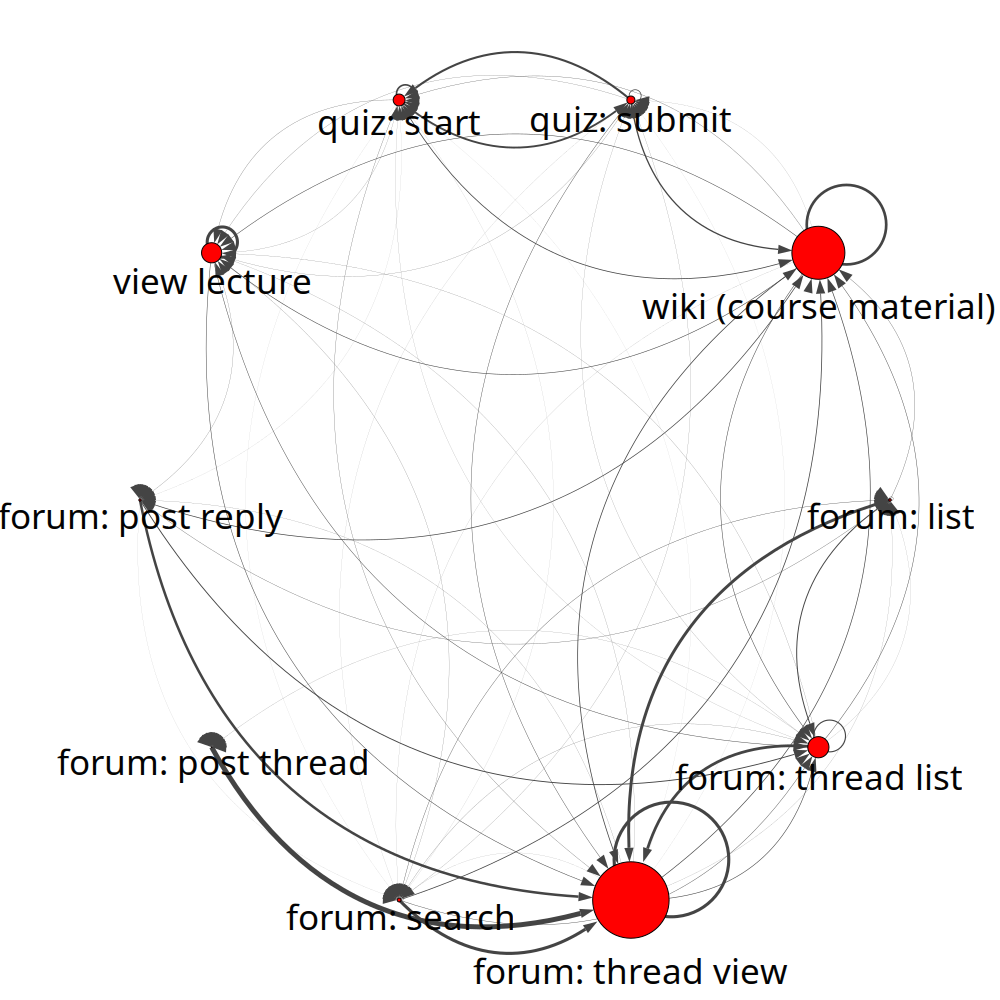
\includegraphics[width=\textwidth]{../../figures/text-4state/state2.png}
            \caption{\label{fig:state2}State 2}
          \end{subfigure}
          \begin{subfigure}[t]{0.9\textwidth}
            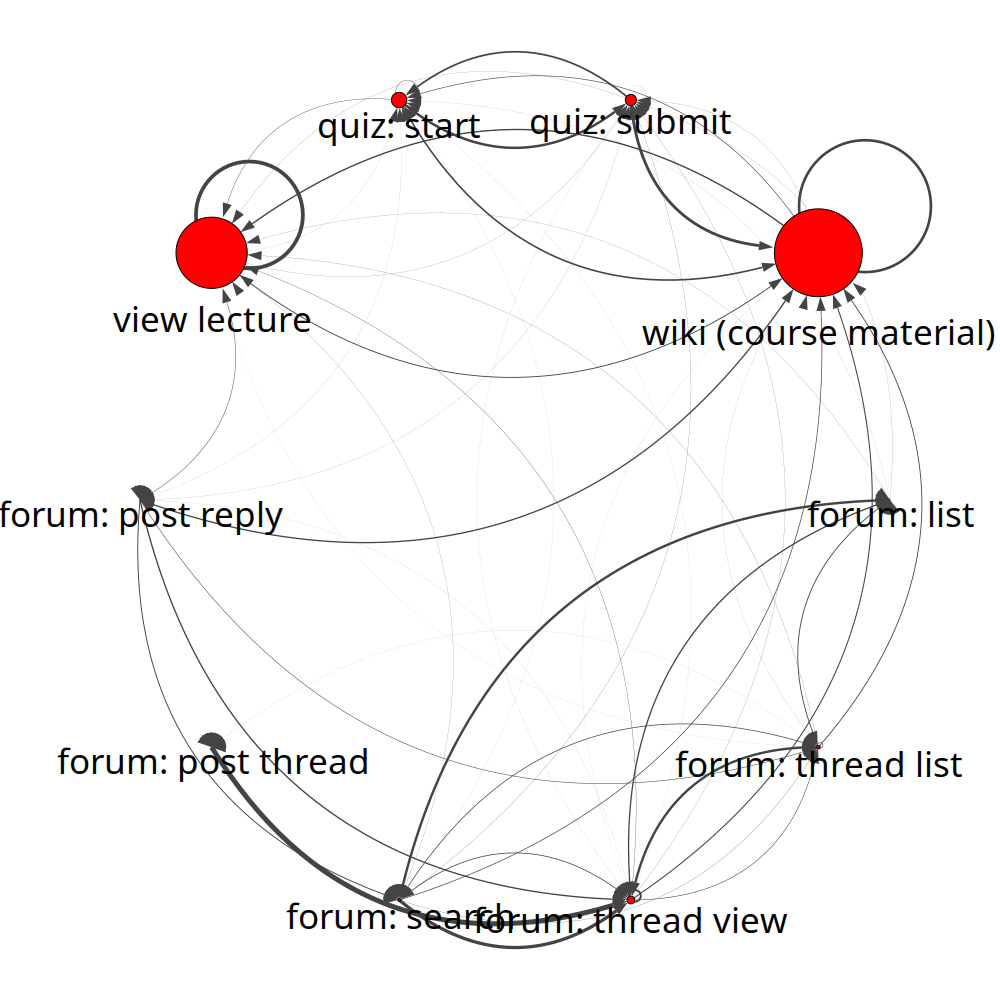
\includegraphics[width=\textwidth]{../../figures/text-4state/state3.png}
            \caption{\label{fig:state3}State 3}
          \end{subfigure}
          \caption{Example states learned by a 4-state TL-HMM on the
          \textretrieval{} MOOC.}
          \label{fig:states}
        \end{figure}
      \end{block}
    \end{column}
  \end{columns}
\end{frame}
\end{document}
